\chapter{Implementace rozpoznávání gest}
Následné algoritmy byly testovány na Kinectu v2 pomocí projectGeneratoru od openFrameworks. Program má i vývojové prostředí, ze kterého to lze spouštět. V přiloženém README.txt bude uveden postup pro generátor pomocí příkazové řádky.

\section{Software}
\subsection{openFramworks}
OpenfFrameworks ~\cite{1} je open source C++ nástroj pro kreativní programování.\\
Využívá se doplněk ofxKinectV2~\cite{2}. Oproti zabudovanému ofxKinect je optimalizovaný pro aktuální openFrameworks (verze 0.9.0), je stabilnější, rychlejší a podporuje pro případné potřeby i více kamer.

Kód v openFrameworks se dělí do třech hlavních částí. Jedná se o setup(), update() a draw(). Sekce setup slouží pro počáteční nastavení programu, proměnných apod., update obsahuje výpočetní a aktualizační část a draw má na starosti vykreslování.

Program se snaží vykonávat všechny části tak často, jak to lze. V update i draw se může využít funkce ofGetElapsedTimef(), která vrací vteřiny v jednotkách float od spuštění programu nebo ofGetElapsedTimeMilis(), která vrací milisekudny od resetování čítače. Pomocí využití modulo funkce (i jiných) můžeme ovlivnit jak často se bude vykonávat každá aktualizační část nebo její podčást, jelikož lze předpokládat, že člověk nemění gesta rychleji, než je počítač zpracovává. Omezení snímků určených ke zpracování programem lze povést i pomocí funkce isFrameNew(), která vrací boolean hodnotu určující, jestli se snímek změnil či nikoliv.

% %\subsection{Měření času v OF}
%timeStart = ofGetElapsedTimef();
%	/*kód*/
%timeEnd = ofGetElapsedTimef();
% %diffTime = timeEnd - timeStart;

\section{Hardware}
\subsection{Kamera Kinect}
K implementaci této práce je využita kamera Kinect v2. Zdroje, ze kterých lze data využít k potřebám aplikace jsou RGB kamera s rozlišením 1920 x 1080 pixelů a kamera na snímání hloubky s rozlišením 512 x 424 pixelů.

Jedná se o relativně levnou a dostupnou kameru, která se v době zpracování této práce (začátek roku 2018) dá pořídit do tří tisíc korun.

\section{Zpracovatelné vstupy}

Obě kamery mohou poskytovat užitečné informace pro účely projektu. RGB kamera nabízí pole pixelů, kde každý má složky RGB (0 až 255). Lze využít v kombinaci s robustním programem, který by na základě barvy, tvarů a dalších vylučovacích prvků správně detekoval nejdříve ruku a poté i gesta. Jedná se o znatelně náročnější způsob.

Hloubková kamera poskytuje pole s hodnotami 0 až 255 dle vzorce pro výpočet vzdálenosti na základě doby letu infračerveného světla. Stupnice hodnot je klesající, to jest nejbližší objekty mají hodnotu 255. Ve vzdálenosti 3 metry hodnoty klesnou na 150. 

\begin{figure}[htp]
\centering
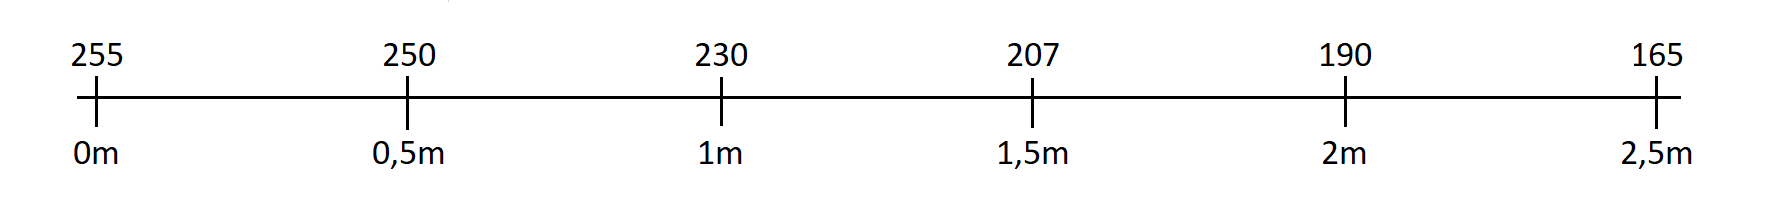
\includegraphics[width=\textwidth]{scale.png}
\caption{Stupnice hodnot, kterých nabývá hloubková kamera v závislosti na vzdálenosti}
\label{fig:scale}
\end{figure}

Minimální vzdálenost pro správné měření vzdálenosti je 0.5 m a maximální 4.5 m. Při větší vzdálenosti bude Kinect stále ještě detekovat věci v zorném poli, ale bude poskytovat nepřesná data a hloubková kamera pozbydu užitku. Velký vliv má i rozlišení, které je pro velké vzdálenosti nedostačující. V dálce 5 m od kamery je rozlišení 7 cm.

Využitelné parametry:

\begin{itemize}
\item Vzdálenost od kamery
\item Vzdálenost mezi pixely
\item Úhly
\item Barvy pixelů
\end{itemize}

\subsection{RGB video}
Zpracování obrazu z RGB videa nebude v této práci implementováno, ale patří do jedné z variant, jak detekovat ruku a následně i gesta.\\
komentář: nejsem si jistá, jestli to sem patří, ale do osnovy/obsahu práce to vytváří kompletnější dojem

\subsection{Hloubkové video}
Doporučený postup by měl sestávat ze čtyř částí:

\begin{enumerate}
\item Úvodní nastavení
\item Nalezení ruky
\item Identifikace gesta
\item Vykreslení ruky (volitelné)
\end{enumerate}

\subsubsection{Úvodní nastavení}
Lze zde dát uživateli na vědomí podmínky interakce s kamerou. Například pozice ruky musí být v prostřední třetině. Alternativou může být počáteční umístění ruky doprostřed kamery, aby mohla dále vycházet z umístění za využívání historie nebo aby se zkrátila doba hledání ruky. V této aplikaci je nejen počátečná podmínkou, že ruka musí být nejbližší objekt před kamerou.

\subsubsection{Nalezení ruky}
Jedná se o prostor pro určení podmínek a způsobu vyhledávání ruky. Tato část rozhoduje o robustnosti kódu a využitelnosti aplikace. Je vhodné nejdříve odstranit nulové a jinak nevyhovující pixely, vyplnit díry v obraze a počítat s dalšími chybami hardwaru a vlivy okolí. Pokud má být aplikace využívaná v jakkoliv náročnějším okolí, musí obsahovat i vyloučení veškerých nevyhovujícíh objektů, jako jsou věci podobného tvaru či případně cizí ruce.

Předpoklad pro následující text je zpracování videa ohledně nulových pixelů. Měly by být ignorovány v rámci chybného vstupu. Zároveň platí, že čím více podmínek se uživateli na začátku předloží, tím jednodušší je nalezení ruky. 

U správně ukazovaného gesta se dá předpokládat stejná vzdálenost jednotlivých bodů od kamery. Mírné odchylky se dají buď zahrnout offsetem, který rozdíly v určitém rozmezí bude považovat za ekvivalentní. nebo vyloučit úplně, jelikož se dá předpokládat, že to nebude mít vliv na zpracování, pokud se jedná o krajní body. Aby byl program uživatelsky přívětivý, v programu je zvolena odchylka na zachycení těchto rozdílů.

V tomto programu se vychází z předem definované vzdálenosti, ve které je nalezen největší možný čtverec, který by představoval dlaň. Pro účely nalezení by muselo existovat pole pixelů, které by reprezentovalo dlaň, či případně podobný objekt, který by se následně vyloučil podle dalších kritérií. Nadále by byla dlaň definovaná středem nalezeného čtverce a šířkou.

Následuje vylučování mylných objektů podle toho, jak robustní program má být a v jak obtížném prostředí bude detekce probíhat. Tato část je předmětem budoucích rozšíření, jelikož se jedná o komplexní problematiku.

Nutnou podmínkou ruky je, že obsahuje prsty, které mají proporcionálně ke dlani určitou velikost a vzdálenost od středu dlaně. Jelikož známe střed nalezené dlaně, lze identifikovat i prsty, respektive konečky prstů. Ze začátku musí být známo jaké gesto bude ruka zobrazovat při inicializaci, aby se dala nalézt. Pro ilustraci bude rozebráno gesto se všemi prsty nataženými. 

Nejjednodušší metodou je nalezení lokálních maxim po šíři dlaně. Když se dlaň rozdělí na čtyři části a v každé se nalezne maximum po ose y (ose x pro horizontální polohu ruky), pro každý prst se změří vzdálenost špičky prstu od středu dlaně. Pokud se bude výrazně odchylovat od proporcí běžné ruky, bude nalezený objekt vyloučen.

Rafinovanější programy využívají tvorbu skeletonu pro sledování a identifikaci jak postavy, tak i ruky. Jedná se o postup nalezení kostí a jejich kloubů, které jsou reprezentovány čárami, což pak reprezentuje ruku (případně tělo). Jedná se o možný, ale mírně náročnější a zdlouhavější postup.

\subsubsection{Identifikace gesta}
Výběr jednotlivých gest je vhodno prodiskutovat s jejich potenciálními uživateli a rozhodnout se mezi dynamickými a statickými gesty. Případně by obě možnosti šly kombinovat, ale byl by to zbytečně komplikovaný postup. Pro gesta dynamická je potřeba udržovat si v paměti minulé stavy a stanovit dobu, po kterou by bylo přijatelné pro uživatele provádět gesto a zároveň to nemohlo být zaměnitelné nebo mylně identifikované. Nejjednodušší je identifikovat gesta statická, kde s využitím souřadnic lze vypočítat počet prstů, a tak v základní verzi bude prostor pro minimálně pět variant, pokud se pro zjednodušení vyloučí zavřená pěst. V momentě, kdy bude program podporovat identifikaci jednotlivých prstů od sebe, je k dispozici variant hned více, než by kdy bylo třeba nebo by bylo zapamatovatelné pro uživatele.

Počet prstů lze vypočítat po správné identifikaci jednotlivých prstů, a jedná se o nejjednodušší způsob klasifikace gesta. Pro přesnost se lze opřít i o úhly a vzdálenosti mezi středem dlaně a špičkami prstů podle vzorců uvedených v kapitole 2.1.4 u obrázku 8.

Sledování gesta může také probíhat pomocí ukládání historie. Za předpokladu, že se člověk hýbe pomaleji, než se střídají snímky k analýze, lze procházet menší část pole, například jen okolí místa, kde se posledně nacházela ruka s prsty a kontrolovat změny, zda počet ukázaných prstů se zmenšil nebo zvětšil. K tomuto účelu by stále stačilo gesto definované počtem prstů bez závislosti na tom, o které konkrétně se jedná.

Otázkou je i jaký objekt má představovat gesto. Jedná-li se o číslo, je to nejjednodušší. Může to být ale i objekt, který obsahuje pět prstů, z nichž každý může být zvednutý nebo nikoliv. Pak je podstatně přehlednější implementace více než pěti gest. Identifikace je ale náročnější, jelikož každý nalezený prst se musí nejdříve identifikovat, poté aktualizovat objekt představující ruku před kamerou a porovnat s implementovanými gesty. 

\subsubsection{Vykreslení ruky}
Objekty se přes video vykreslují pomocí FBO ("frame buffer object"). Jedná se o buffery s objekty, které je třeba vykreslit. Reprezentují plátno, na které se pomocí pomocí příkazů 'begin()' a 'end()' vykreslují 3D objekty a jednou za snímek či méně často (podle požadavků) se vykreslí pomocí příkazu 'draw()'. Pro lepší přehled se můžou jednotlivé prsty (konečky prstů) zvýraznit koulí, zatímco celá ruka krychlí. Vykreslují se pouze základní objekty, které upřesňují nalezenou pozici rukou a prstů, aby nebylo potřeba udržovat v paměti přesné okraje ruky, které ani nejsou potřeba.

\section{Předzpracování}

Kvůli přehlednější práci s matematickými parametry obrazu se nejdřívnačte video, které je uloženo v 1D poli do 2D pole pro další zpracování.\\

\subsection{Filtrace}
Jelikož se do obrazu dostane značné množství chybných hodnot, je potřeba je nejdříve co nejvíce eliminovat. Za tímto účelem je použit medián z okolí. Kvůli překreslování aktuálních hodnot jsou pro dalš výpočty použita data z pole zrcadlícího originální data. Pro každý pixel je načteno okolí o požadované velikosti, které se seřadí podle velikosti a jako výsledná hodnota se vezme hodnota z prostřední pozice.\\

Velikost okolí by se měla vybrat empericky. Čím větší okolí, tím více je výsledek rozmazaný, ale zato obsahuje menší počet odchýlených hodnot, které by mohly narušit průběh zpracování. Pokud se vezme okolí malé, zůstane jich více, ale lépe se zachovají tvary. Na následujících obrázcích lze pozorovat rozdíl mezi okolím 9 (obrázek 9) a okolím 25(obrázek 10).\\

\begin{figure}[htp]
\centering
\fbox{\includegraphics[width=.4\textwidth]{3-neigh9/befOUT.png}} \hfil
\fbox{\includegraphics[width=.4\textwidth]{3-neigh9/afOUT.png}}
\caption{Medián vzatý z okolí mohutnosti 9 \\ a) originální obraz b) po úpravě}
\label{fig:neigh9}
\end{figure}
\begin{figure}[htp]
\centering
\fbox{\includegraphics[width=.4\textwidth]{4-neigh25/befOUT.png}} \hfil
\fbox{\includegraphics[width=.4\textwidth]{4-neigh25/afOUT.png}}
\caption{Medián vzatý z okolí mohutnosti 25 \\ a) originální obraz b) po úpravě}
\label{fig:neigh25}
\end{figure}

\subsection{Prahování}
Pro manipulaci s nalzenými tvary a výpočty mezi jednotlivými body je snazší pracovat s binárním obrazem. Nejdříve se obraz projde a najde nejbližší objekt (největší hodnota). Díky předchozí filtraci nezkreslí tuto hodnotu žádný špatně naměřený pixel. Následně se již porovná každý jednotlivý pixel s hodnotou a vytvoří se pole s hodnotami 1 a 0.

Jelikož lze předpokládat, že člověk nebude mít vždy ruku striktně kolmo k pohledu kamery, je záhodno odečíst od této hodnoty odchylku. Výsledná hodnota tedy záleží na tom, zda původní pixel byl blíže, než nejbližší objekt s ohledem na odchylku.\\
Na obrázcích 11, 12 a 13 lze pozorovat změny s ohledem na různé tolerance naklonění ruky. S odchylkou 10 vidíme, že ještě kus dlaně chybí, při odchylce 15 je s rukou načtený i znatelný kus předloktí a k tomu i nejednotný kus jiného objektu. Při toleranci pouze 12 je stále načteno moc pixelů a tak se jeví 10 jako nejvhodnější tolerance.\\

\begin{figure}[htp]
\centering
\fbox{\includegraphics[width=.3\textwidth]{5-depth-10/befOUT.png}} \hfill
\fbox{\includegraphics[width=.3\textwidth]{5-depth-10/afOUT.png}} \hfill
\fbox{\includegraphics[width=.3\textwidth]{5-depth-10/binOUT.png}}
\caption{Prahování s odchylkou 10 \\ a) originální obraz b) po filtraci c) binární obraz}
\label{fig:tresh10}
\end{figure}
\begin{figure}[htp]
\centering
\fbox{\includegraphics[width=.3\textwidth]{7-depth-12/befOUT.png}} \hfill
\fbox{\includegraphics[width=.3\textwidth]{7-depth-12/afOUT.png}} \hfill
\fbox{\includegraphics[width=.3\textwidth]{7-depth-12/binOUT.png}}
\caption{Prahování s odchylkou 12 \\ a) originální obraz b) po filtraci c) binární obraz}
\label{fig:tresh11}
\end{figure}
\begin{figure}[htp]
\centering
\fbox{\includegraphics[width=.3\textwidth]{6-depth-15/befOUT.png}} \hfill
\fbox{\includegraphics[width=.3\textwidth]{6-depth-15/afOUT.png}} \hfill
\fbox{\includegraphics[width=.3\textwidth]{6-depth-15/binOUT.png}}
\caption{Prahování s odchylkou 15 \\ a) originální obraz b) po filtraci c) binární obraz}
\label{fig:tresh12}
\end{figure}
\section{Detekce ruky}
Definujeme-li ruku jako nejbližší objekt, pak již při prahování je nalezena. Pro lepší názornost se ukládá umístění objektu pomocí pole souřadnic. Na videu je vizualizován pomocí červeného čtverce, který má střed v zprůměrovaných souřadnicích (Xavg, Yavg) a velikost odvozenou od velikosti pole. 
Na následujících obrázcích je vidět rozdíl mezi vyhledáváním v originálních datech a nebere v potaz chybné hodnoty a vyhledáváním v binárním obraze s vyfiltrovaným šumem.
\begin{figure}[htp]
\centering
\fbox{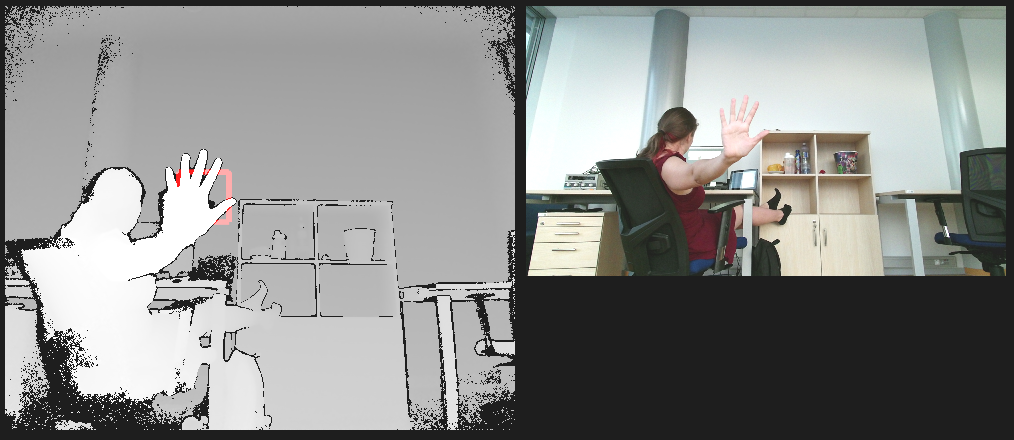
\includegraphics[width=.8\textwidth]{inDepth.png}}
\caption{Obrázek ukazuje největší nalezený nejbližší objekt z originálních dat.}
\label{fig:square_depth}
\end{figure}
\begin{figure}[htp]
\centering
\fbox{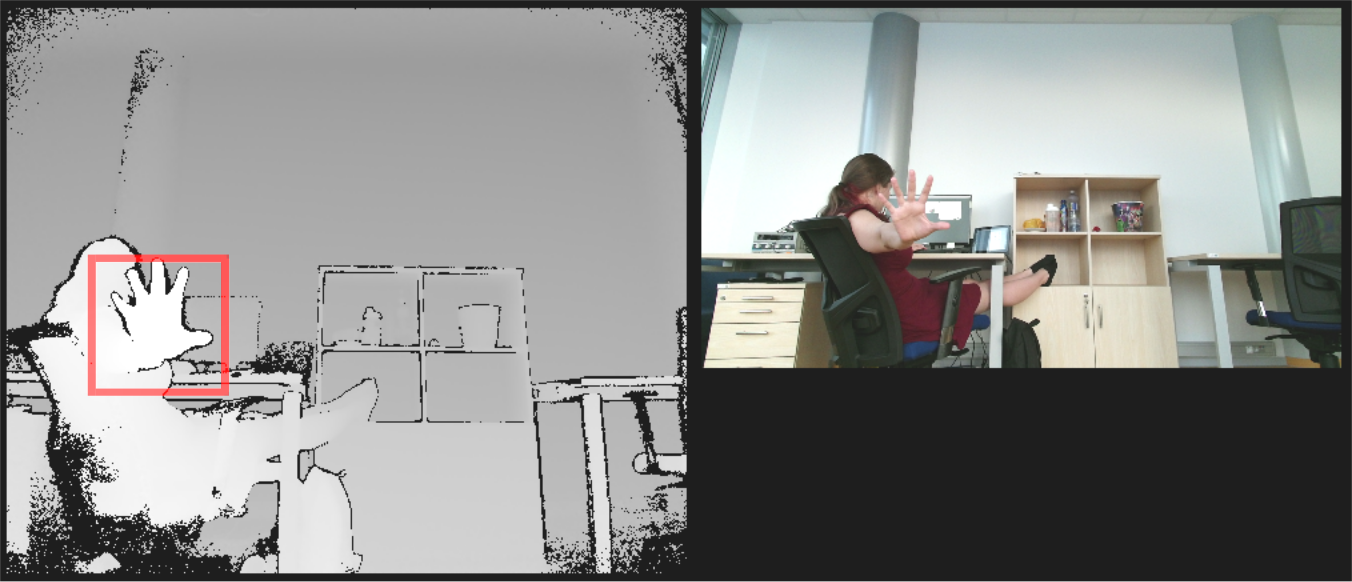
\includegraphics[width=.8\textwidth]{inBinary.png}}
\caption{Největší nejbližší objekt nalezený v binárních vyfiltrovaných datech.}
\label{fig:square_bin}
\end{figure}

Již z obrázků lze poznat, že vyhledávání v binárních datech je přesnější.

\section{Detekce dlaně}
V binárním obraze se vyhledá největší čtvercová matice, kterou lze považovat za dlaň. Vytvoří se pomocné matice, do které se zapíší krajové hodnoty binárního obrazu a poté se binární pole prochází z levého horního rohu.\\
Pokud je na dané pozici binárního obrazu nula, přepíše se i do matice. Pokud je tam ale jedna, pak se nalezne minimum třech sousedů z levého horního rohu. K minumu se přičte daná jedna, čímž se zvětší velikost čtvercové matice. Ve výsledku tak největší číslo, které je nalezené v pomocné matici, představuje pravý dolní roh největší matice a zároveň její velikost~\cite{23}.
\begin{figure}[htp]
\centering
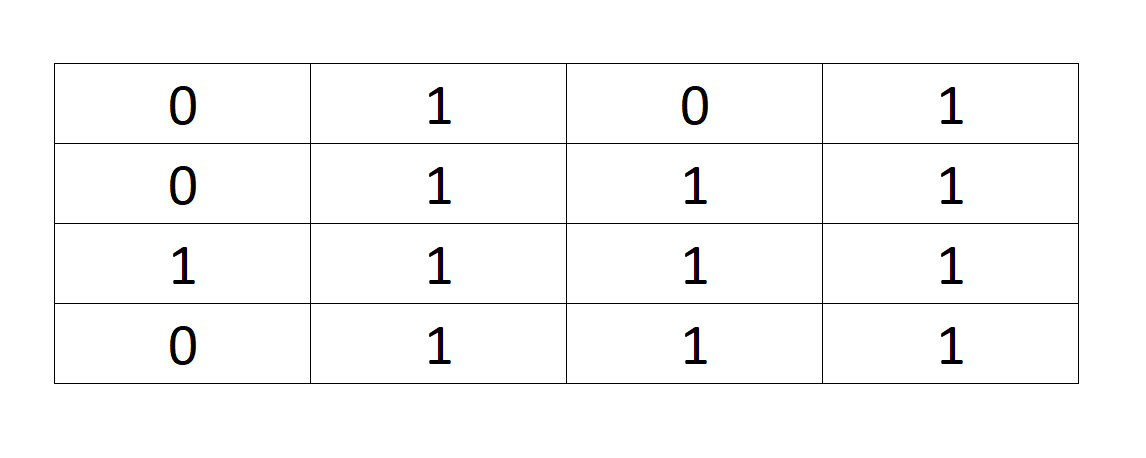
\includegraphics[width=.45\textwidth]{before.png} \hfill
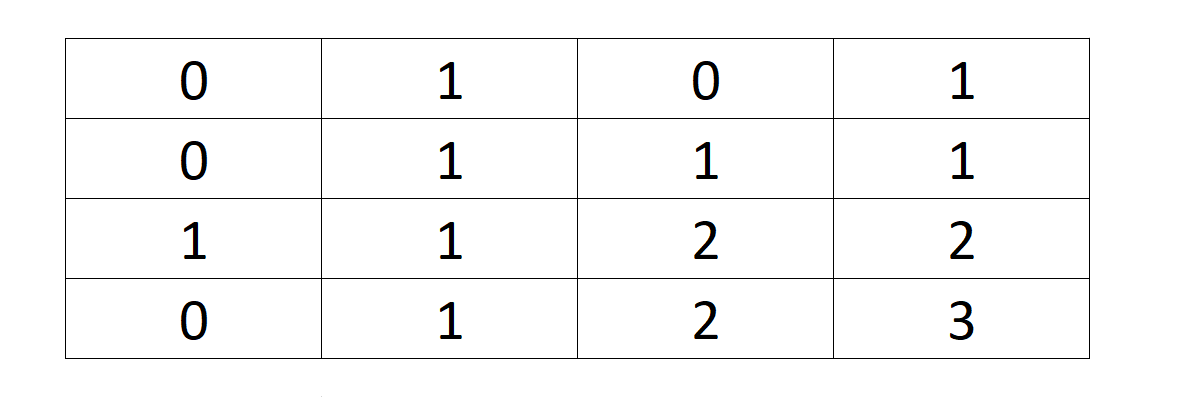
\includegraphics[width=.45\textwidth]{after.png} 
\caption{Nalezení největší jednotkové matice v binárním obraze.}
\label{fig: palm}
\end{figure}\\
Vykresluje se pomocí zeleného čtverce, jenž má velikost nalezené jednotkové matice a jeho střed má souřadnice Xc, Yc, které budou následně využívány jako střed dlaně.

\begin{figure}[htp]
\centering
\fbox{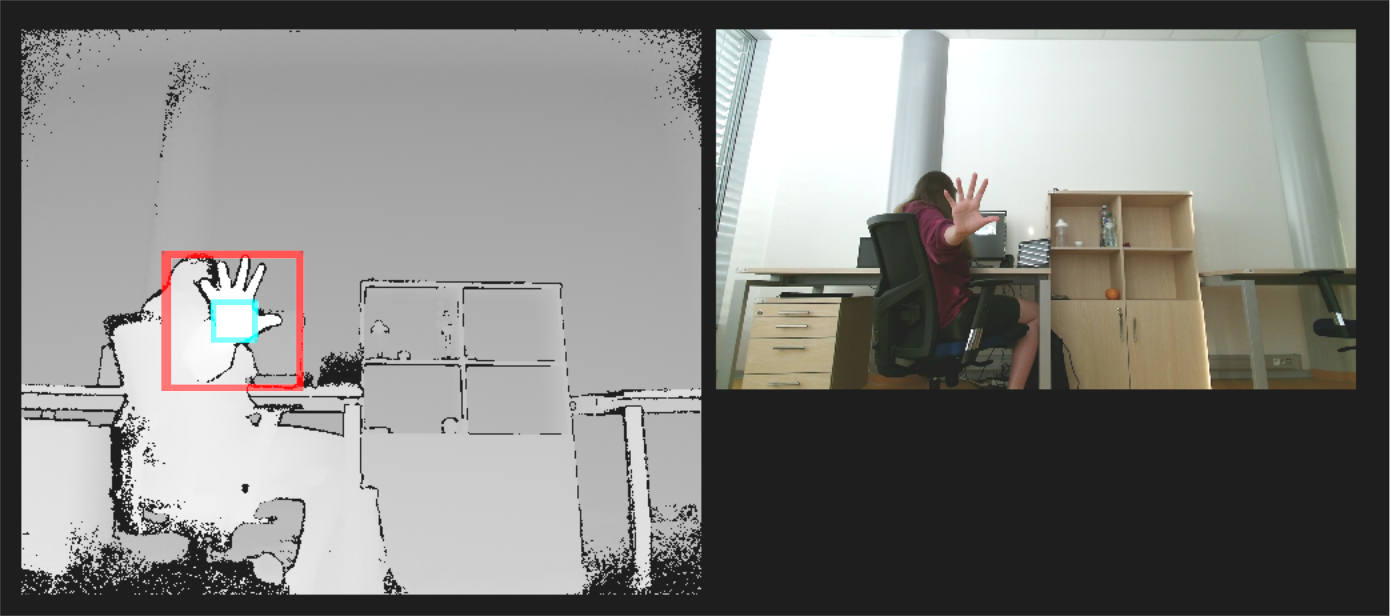
\includegraphics[width=\textwidth]{square.png}}
\caption{Červený čtverec znázorňuje polohu a velikost nalezeného nejbližšího objektu.\\
Zelený čtverec obkresluje největší nalezený čtverec v objektu.}
\label{fig:square}
\end{figure}

\section{Detekce prstů}
V aplikaci je implentováno několik způsobů nalezení prstů. Ne všechny jsou efektivní a od některých se upustilo (viz kapitola statistika), ale pro různost postupu jsou zde uvedeny.

\subsection{Detekce směru prstů}
Za předpokladu, že jsou prsty nezaměnitelně hubenější, než předloktí, lze okolo dlaně ve vzdálenosti $ offset\_palm $ od okraje vést čáru ve všech čtyřech směrem. Následně se iteruje podél jednotlivých čar a detekují změny v binárním obraze a zaznamenává se počet předpokládanách prstů. Jelikož je potřeba znát i pozici palce, ukládají se dva směry prstů.

Empiricky nalezená nejlepší hodnota pro $ offset\_palm $ je $ \frac{5}{7} $ šířky dlaně. 

\begin{figure}[htp]
\centering
\fbox{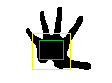
\includegraphics[width=.4\textwidth]{whereFingersAt.png}}
\caption{todo Popisek.}
\label{fig:whereFingers}
\end{figure}

\subsection{Detekce konců prstů}
Všechny postupy se zakládají na prohledávání v okolí dlaně. Maximální délka prstů se odvozuje od nalezené velikosti dlaně. Prsty nesmí být ani příliš dlouhé ani příliš krátké.\\

%findFingerTips
Nejjednodušší postup spočívá v rozdělení strany, na které se nachází prsty, na čtyři části, kde každá náleží jednotlivým prstům. Rozdělení je rovnoměrné a nepodporuje tak extrémní odchylky. Celkový obdélník musí být širší než dlaň a nebere se v potaz, který prst je v daném obdélníku nalezen. To znamená, že pokud se ukazují dva prsty, přičemž se některý/oba nachází ve vedlejším obdélníku, zaznamená se správně pouze počet prstů.

Jednotlivé části se následně procházejí a hledá se pixel, který ještě patří prstu a je nejvýše/nejníže dle orientace.\\

\begin{figure}[htp]
\centering
\fbox{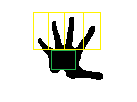
\includegraphics[width=.4\textwidth]{findFingerTips.png}}
\caption{todo Popisek.}
\label{fig:findFingerTips}
\end{figure}

%findFingerTips2
Další způsob zvyšuje použitelnost předchozí metody. Stále se prochází pole, ale celkový obdélník se předá v kuse a hledá se největší vzdálenost od středu dlaně. Stále platí omezení délky, tudíž je přesnější největší možná vzdálenost, která stále patří prstu.

%findFingerTips3
Funkce findFingerTips3 si ukládá souřadnice, na kterých byly detekovány prsty z předchozí kapitoly. Následně si dopočítá střed prstu a po přímce prohledává binární obraz tak daleko, dokud nenarazí na konec prstu (nulu v binárním obraze). 

\section{Statistika}
Vyhodnocení funkčnosti a použitelnosti navržených metod.

\endinput
%%
%% End of file `ch01.tex'.
